\subsubsection{Site Overview}\label{overview}
Si fa riferimento alla pagina: \\
\url{http://www.alexa.com/siteinfo?ax_atid=3dcecff3-eaba-4eb2-98d8-af635c113373}
\begin{figure}[ht]
\centering
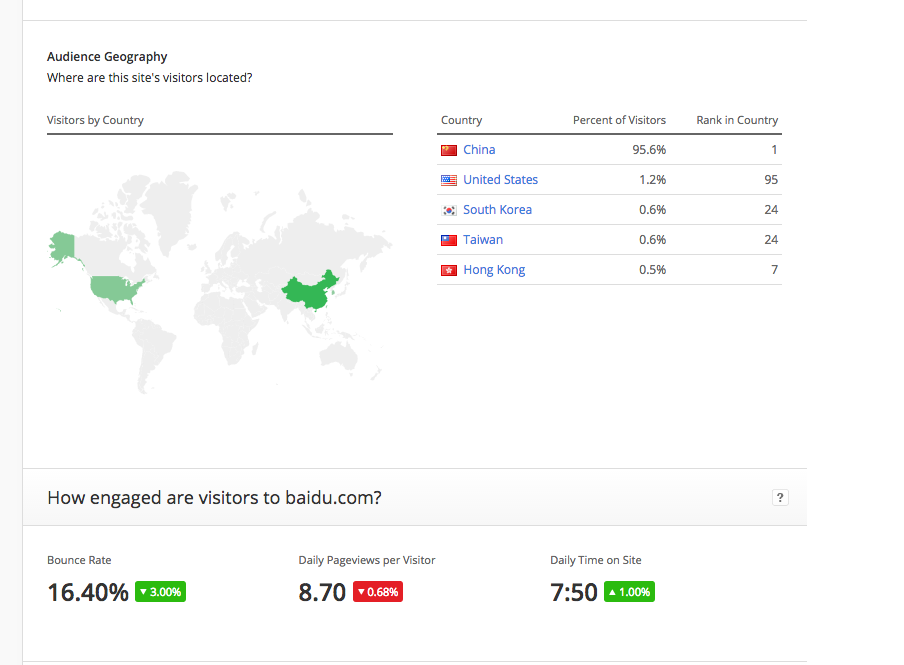
\includegraphics[scale=0.4,keepaspectratio]{{figure/4/siteOverviewSearch1}.png}
\caption{Pagina Site Overview (primo scroll) - presentazione dei risultati di ricerca}
\end{figure}
\FloatBarrier
Altri screenshot relativi alle schermate di scroll contenute in questa
pagina sono disponibili ai path:
\begin{itemize}
	\item \textit{figure/4/siteOverview0.png}
	\item \textit{figure/4/siteOverview2.png}
	\item \textit{figure/4/siteOverview3.png}
	\item \textit{figure/4/siteOverview4.png}
\end{itemize}
La pagina permette di provare alcune funzionalità ristrette del motore di 
ricerca in modo che l'utente possa farsi un'idea dei vantaggi 
che lo strumento offre. \\
Utilizzando la barra di ricerca è possibile indicare un sito web di cui 
si vogliono calcolare le metriche. \\
La prima pagina di risultati (siteOverview0.png) mostra il traffico rispetto
agli altri siti e la posizione in Alexa Rank rispetto alla nazione di punta ed al
resto del mondo. Scrollando altre pagine si possono trovare informazioni
più dettagliate (i.e. distribuzione dei visitatori per nazione, keyword 
utilizzate per trovare il sito, altri siti visitati poco prima di approdare
al sito, pagine interne più visitate, siti correlati, distribuzione dei
visitatori divisi per occupazione etc.). I contenuti sono presentati in modo
molto efficace (grafici, percentuali, classifiche in liste numerate), 
in questo caso è 
accettabile lo scrolling perch\'e le informazioni sono difficilmente
frazionabili. Si potrebbe comunque dividere il contenuto per 
tipologia di metrica inserendo ogni
sottosezione di scrolling in una lista verticale (ogni elemento 
identificato da un titolo) che mostri
solo il primo elemento lasciando all'utente la scelta di quale
elemento esplodere secondo le sue necessità. Così si elimina lo scrolling ed il contenuto viene presentato in una forma più compatta e navigabile.  
Una critica riguarda il fatto di non
sfruttare tutto lo spazio della pagina (stessa critica fatta ad Homepage):
si potrebbero espandere i contenuti (soprattutto i grafici) allargando le 
informazioni in modo che occupino tutto lo spazio disponibile senza lasciare 
colonne vuote ai margini.\\
Risultato : \textit{7.5}